\documentclass[a4paper,12pt]{article}
\usepackage{flafter,epsf}       
\usepackage{amsmath}
\usepackage{amsfonts,amsbsy,amssymb,bbm}
\usepackage{amsthm}  %% proof enviroment
\usepackage{natbibOrig}

\sloppy 
\usepackage{graphicx}
\bibliographystyle{natbib}

% Using the following to mark changes for review
\usepackage{color}
\definecolor{blue}{rgb}{0,0,1}
\newcommand{\mc}[1]{\textcolor{blue}{#1}}
%\newcommand{\mc}[1]{#1}   % Replace above line with this to eliminate all coloring

\input{epsf}

\newcommand {\rel} {\mathbb{R}}
\newcommand {\com} {\mathbb{C}}
\newcommand {\nat} {\mathbb{N}}
\newcommand {\rat} {\mathbb{Q}}
\newcommand {\ganz} {\mathbb{Z}}
\newcommand {\indicator} {\mathbbm{1}}

\newtheorem{defi}{Definition}
\newtheorem{theo}{Theorem}
\newtheorem{corol}{Corollary}
\newtheorem{prop}{Proposition}
\newtheorem{example}{Example}
\newtheorem{lemma}{Lemma}
\newtheorem{problem}{Problem}[section]

\textheight 21cm
\textwidth 16cm
\oddsidemargin -0.1cm
\evensidemargin -0.1cm

\newlabel{sensitivityFig}{1}



\begin{document}

\title{PEACE: {\underline P}arallel {\underline E}ST {\underline A}nalysis
  and {\underline C}lustering {\underline E}ngine \\Supplementary
  Materials}

\date{}

\maketitle  

\begin{appendix}

\renewcommand{\theequation}{S\arabic{equation}}
\renewcommand{\thefigure}{S\arabic{figure}}
\renewcommand{\thetable}{S\arabic{table}}
\setcounter{equation}{0}

\section{Distance metrics, heuristics and filters}

\subsection{The $d^2$ distance metric}
$d^2$, as outlined by {\it Hide et al.} [\cite{Hide94}], is an {\it
  alignment free} distance pseudo-metric which quantifies local
similarity between sequences based on a simple word count.  Let
$c_x(w)$ denote the number of times word $w$ occurs in string $x$.  We
search for similarity between strings $x$ and $y$ by looking at the
difference between $c_x(w)$ and $c_y(w)$ for different words $w$.
Specifically,  for all words of a fixed length $k$, we calculate:
\begin{equation*}
d^2_k(x,y) = \sum_{|w|=k}(c_x(w) - c_y(w))^2
\end{equation*}
However, applying such a definition to two sequences as a whole leads
to a measure of global similarity, while we want to measure local
similarity (thus, for example, assigning two sequences with
sufficiently long overlapping ends to be at a distance of zero -- or a
small distance if errors are present).  For this, instead of comparing
the entire two strings, we compare sliding windows from each string of a fixed
size $r$.  Formally, for sequences $x$ and $y$ ($|x| \geq r$, $|y|
\geq r$), we define:
\begin{equation}
\label{d2def}
d^2(x,y) = 
\min\left\{d^2(u,v) \; : \; u \sqsubseteq x, v \sqsubseteq y, |u|=|v|=r\right\}
\end{equation}
(where $u \sqsubseteq x$ denotes that $u$ is a substring of $x$).
Defined as such, $d^2$ is, in a mathematical sense, a {\it
  pseudo-metric}: $d^2(x,y) = 0$ does not imply $x=y$.

The \textsc{peace} implementation of $d^2$ was initially based on the description from
{\it Hazelhurst} [\cite{Hazelhurst04}].  For parameters
we adapted those used by the \textsc{wcd} clustering tool [\cite{Hazelhurst08a}]:
a word size $k=6$ and a window size $r=100$.

\subsection{Two-pass $d^2$}
Our ``two-pass $d^2$'' algorithm works by sampling a subset of window
pairs evenly distributed across the sequences, narrowing down a
smaller region in which to search for the best scoring window-pair.
In the first pass, the algorithm look at every length $r$ window on one sequence,
but on the other sequence we skip the window by $s$ bases between
every sampling.  It then take the best such window pair, extend
each of these two windows by $s$ bases in each direction, and apply
(\ref{d2def}) to this limited region.

In \textsc{peace}, we use $k=6$, $r=100$, and $s=50$.

\subsection{Filtering heuristics}
\textsc{peace} uses the $u/v$ and $t/v$ heuristics, roughly as described by {\it
  Hazelhurst et al.} [\cite{Hazelhurst08a}] as filters that allows us to avoid
over 99\% of the potential $d^2$ calculations.  Each heuristic takes two
sequences and estimates whether it is worth proceeding to the $d^2$
computation by sampling and comparing word frequency across the two
sequences.  The $u/v$ heuristic looks at every $h$-th word of size $v$
on one sequence, and rejects if it does not find at least $u$ occurrences
of these words on the other sequence.  The $t/v$ heuristic demands
that there be at least $t$ size $v$ words on one sequence that occur
within a $l$ base range within the second sequence.  If a sequence
pair meets the requirements of both these filters, then we compute the
$d^2$ distance.

In \textsc{peace}, we set $h=16$, $v=8$, $u=4$, $t=65$, and $l=100$.

\section{MST-Based  Calculations}

While $d^2$ serves to quantify sequence distance, the basis for the
clustering algorithm is the minimum spanning tree (MST).  Viewing the
ESTs as nodes and the data set as an $d^2$-weighted graph, the
derivation of a minimum spanning tree results in the placement of
nodes of a given tree into a restricted neighborhood of the graph.  By
then removing larger edges, we are left with connected components
corresponding to the gene-based clusters.  The MST-based clustering
method has been used effectively in other applications, but to our
knowledge this is the first such use for the  EST
clustering problem [\cite{Jain99,Wan08}].

\subsection{Calculation of the MST}

To calculate this MST we use Prim's algorithm [\cite{Prim57}].  For a
graph of $n$ nodes and $e$ edges, Prim's can be implemented such that
the algorithm has an $O(e + n \log n)$ worst-case runtime.  However,
the {\it narrow-band} nature of the model allows us to reduce this
bound.  If we were to model only the edges connecting adjacent nodes,
we would find the node degrees to be very small relative to $n$: any
EST overlaps only a few others, and has no connection to a vast
majority of the data set members.  Since we can quickly eliminate most
of these excess edges with the $u/v$ and $t/v$ heuristics (removing
more than 99\% of all edges before applying Prim's), we find in
practice that $e$ is a very small fraction of $n^2$.  In the
runtime results (see Section~\ref{rt_section} and
Figure~\ref{seq_runtime}), we find that when holding the EST size
distribution constant, the tool as a whole has a runtime of $O(n^2)$
-- appearing to dominated by the time required to apply
the filtering heuristics to every EST pair.

\subsection{Removing edges}

Once the MST is has been calculated, our last step is to remove all
edges exceeding a threshold weight $T$, taking the resulting
components as our clusters.  \textsc{wcd}, when faced with a similar
challenge, sets the threshold at $T=40$, hypothesizing that EST pairs
with a $d^2$ distance of greater than 40 are unlikely to overlap.  We
have set out threshold to $T=130$.



\section{Simulated Test Results}

In {\it Hazelhurst et al.} [\cite{Hazelhurst08a}] the authors conduct
an investigation of \textsc{wcd} against a number of clustering
tools.  As they make a convincing argument that \textsc{wcd} is returning
better results then the tools against which they compare, we limit our
analysis to a comparison of \textsc{peace} against \textsc{wcd} and the \textsc{cap3} assembly
tool [\cite{Huang99}] -- a tool which implicitly clusters while
performing assembly.  We do so by applying all three tools to a number
of data sets, both simulated and real.

\subsection{Simulation Tool and Parameters}

For simulated data sets we use the {\bf ESTsim} tool to generate
simulated EST data sets [\cite{Hazelhurst03}], using the collection of
zebra fish genes that served as a basis for the \textsc{wcd} simulations
[\cite{Hazelhurst08a}].  In generating the ESTs, ESTsim models three
types of error (general base read errors, errors due to
polymerase decay, and primer interference), and allows those errors to
take the form of substitutions, deletions, and insertions (of bases
and Ns).  See the paper for a discussion of the probability
distributions and default parameters.  For generating our simulated
data, we use the default values for all parameters that are not
explicitly being subjected to variation in our experiments --
paralleling the testing of the \textsc{wcd} tool.



\subsection{Methodology} 

Each estimate given in the main paper, or in the following, is
averaged over 30 trials.  Each trial consists of the application of
all three tools to a simulated data set, the set having been derived
from the application of the ESTsim tool to a set of 100 zebra fish
gene sequences [\cite{Hazelhurst03}].  All confidence intervals are
calculated at a 95\% level of significance.

\subsection{Result Quality}

While our primary measurement of tool result is sensitivity
(Figure~\ref{sensitivityFig}), a number of alternative measurements
were investigated as well. The {\it Jaccard} index measures both
sensitivity and specificity, calculated as the ratio of true positives
to the sum of true positives, true negatives, and false positives ($tp
/ (tp+fn+fp)$) [\cite{Hazelhurst08a}].  Notably, when we removed duplicated genes before
generating the simulated EST sets, we found all three tools to have
100\% specificity: no false positives.  In such a case the Jaccard
Index is identical to the Sensitivity Index, hence \textsc{peace} exhibits the
same improvement on both indexes relative to \textsc{wcd} and \textsc{cap3}.  Applying
the tools to the original genes (in which 21\% of the genes were
highly similar to genes in the remaining 79\%), we find only a slight
difference in the Jaccard Index, and the same relative performance of
the three tools (Figure~\ref{JiSe}).  The sensitivity of each tool to
duplications is discussed below.

%%%%%%%%%%%%%%%%%%%%%%%%
\begin{figure}[tbp]
\centerline{
\includegraphics[scale=0.5]{4JiSe.eps}
\label{JiSe}
}
\caption{Comparisons of Sensitivity and the Jaccard Index as a
  function of base read error rate, based on 30 simulated EST sets
  derived from a set of 79 genes with no significant similarity (left
  column), and an additional 21 genes showing significant similarity
  to the base set (right column).  Blue/Solid = \textsc{peace}, Green/Dash =
  \textsc{wcd}, Black/Dot-Dash = \textsc{cap3}; vertical tics = 95\% confidence
  intervals on estimates.}
\end{figure}
%%%%%%%%%%%%%%%%%%%%%%%%

Type 1 and Type 2 errors, as defined in {\it Wang et al.}
[\cite{Wang04}], measure quality at the level of the genes from which
the ESTs were derived.  For Type 1 error, we look at the fraction of genes
that were  broken into two or more partitions, while in
Type 2 error we look at the fraction of clusters that contain two or
more genes.   In Figure~\ref{t1t2} we compare the Type 1 and Type 2 error rates of
the three tools for varying levels of simulated base read error.  For
Type 1 error we find that while all tools do equally poorly when the
EST is subjected to more than a $5\%$ error rate, \textsc{peace} does
significantly better than \textsc{wcd} in the lower ranges (while
\textsc{wcd} does correspondingly better than \textsc{cap3}).  When
looking at Type 2 error rate, we find that \textsc{peace} does a
generally better job than \textsc{cap3} in separating genes into
different clusters.  We note, however, that Type 1 error is the more
important measurement: genes incorrectly split between clusters cannot
be later recovered (without re-examining the cluster as a whole), but
there is the potential for an assembly program to later identify
incorrectly merged clusters based only on local cluster information.


%%%%%%%%%%%%%%
\begin{figure}[tbp]
\centerline{\includegraphics[scale=0.5]{t1t2.eps}
\label{t1t2}
}
\caption{Type 1 error rate (fraction of genes partitioned) and Type 2
  error rate (fraction of clusters containing multiple genes) as a
  function of base read error rate.  Estimates averaged over
  application to 30 simulated ESTs sets derived from the full 100
  zebra fish gene set. Blue/Solid = \textsc{peace}, Green/Dash =
  \textsc{wcd}, Black/Dot-Dash = \textsc{cap3}; vertical tics = 95\%
  confidence intervals on estimates (not shown for Type 1 error due to
  the extremely small variance in estimates).}
\end{figure}
%%%%%%%%%%%%%%

One of the difficulties in clustering EST data is dealing with
highly similar genes.  Genes with a high degree of similarity will
produce ESTs that reflect that similarity, hence appear to overlap --
resulting in the incorrect clustering of ESTs from separate genes.  Assembly tools
such as \textsc{cap3} may have more ability to discriminate between clusters
given their more intensive investigation of overlaps, but highly
similar sequences are going to cause a problem for any tool. 

In Figure~\ref{dups} we look at the ability of each tool to separate
duplicates as a function of the \% divergence between the
duplications.  Unsurprisingly, \textsc{cap3} (the assembler) does the best
here, able to effectively separate duplicates at $~92\%$ similarity
or less.  \textsc{peace} and \textsc{wcd} are roughly comparable, both clearly able to
separate duplicates out at a similarity level of $83\%$ -- but completely 
unable to distinguish sharing a similarity of $~88\%$ or more. 

\begin{figure}[tbp]
\centerline{
\label{dups}
\includegraphics[scale=0.35]{duplicates.eps}
}
\caption{Ability to distinguish duplicates as a function of
  divergence.  Estimates averaged over 30 trials; one trial consists
  of taking a random gene, copying it and stochastically changing bases
  at the specified rate, then using the two genes as the bases for
  generating a simulated set. Blue/Solid = \textsc{peace}, Green/Dashed = \textsc{wcd}, Black/Dot-Dashed = \textsc{cap3};
  variance was too small for visible plotting of
  confidence intervals.}
\end{figure}

\subsection{Runtime}
\label{rt_section}

In Figure~\ref{seq_runtime} we see give a runtime comparison of \textsc{peace} and \textsc{wcd},
seeing a slight improvement in \textsc{peace}.  (As \textsc{cap3} performs both
clustering and assembly, runtime comparisons are not meaningful.)  As
stated, we see an almost perfectly quadratic curve ($r > 0.99$),
indicating that the runtime is dominated by the time required to look
at every EST pair (either filtering or computing $d^2$).
As both \textsc{peace} and \textsc{wcd} can be run in a parallel mode, we also
examined runtime as a function of the ratio of EST set sizes to number
of processors used.  In Figure~\ref{par_runtime} we show two such ratios,
again seeing an improvement in \textsc{peace} over \textsc{wcd}.

%%%%%%%%%%%%%
\begin{figure}[tbp]
\centerline{
\includegraphics[scale=0.35]{seq_time.eps}
\label{seq_runtime}
}
\caption{Single Processor Runtime as a function of input size,
  averaged over 50 simulated EST sets; Blue/Solid = \textsc{peace},
  Green/Dashed = \textsc{wcd}; vertical tics represent= 95\% confidence
  intervals on estimates.}
\end{figure}
\begin{figure}[tbp]
\centerline{
\includegraphics[scale=0.5]{par_time.eps}
\label{par_runtime}
}
\caption{Runtime of a function of input size when holding constant the
  ratio of set size to number of processors used; averaged over 30
  simulated EST sets.  Blue/Solid = \textsc{peace}, Green/Dashed = \textsc{wcd};
  vertical tics represent= 95\% confidence intervals on estimates.}
\end{figure}
%%%%%%%%%%%%%

\section{Applications to Real Data Sets}

In Table~\ref{chlamy} we lay out more comprehensive results for the
application of our tool to an EST set collected from the {\it
  Chlamydomonas reinhartdii} genome, while in Table~\ref{mouse} 
we see the results for the mouse set used for the \textsc{wcd} analysis
[\cite{Hazelhurst08a}].  We note that for the Chlamydomonas genome the
correct clustering is not known; our estimates of sensitivity are
based on as assignment of ESTs to the sequenced genomes by the Gmap tool
[\cite{Wu05}], leaving some potential for error in the  reference.
Further, we found a number of ligations in the data (ESTs derived by
incorrectly combining multiple transcripts),  which were removed before testing.

Interestingly, where in the simulated results we saw significant
improvement in \textsc{peace} over \textsc{wcd} in terms of result quality and only a
light improvement in runtime, here we see the reverse. The two tools are
roughly comparable  in terms of sensitivity, Type 1 error and Type 2
error, while \textsc{peace} shows a 10\% and 20\% improvement in runtime (both
showing significant improvements over \textsc{cap3}).  Predictably , the full
assembly tool does somewhat better in terms of specificity (the Jaccard
Index and Type 2 error), though scores here are worse for all three
tools due to the increased number of homologous gene pairs as compared
to our simulated sets.

\begin{table}[tbp]
\begin{center}
\begin{tabular} {| c || c | c | c | c | c | c | c | c |}
\hline
& Sensitivity & Jaccard & \begin{tabular}{c} Type 1 \\
  error \end{tabular} & \begin{tabular}{c} Type 2 \\
  error \end{tabular} & \begin{tabular}{c} Number \\ of  \\
    Clusters \end{tabular} & Singletons & \begin{tabular}{c} Single
      \\ processor \\ runtime (s) \end{tabular}\\
\hline \hline \textsc{peace} & 0.958 & 0.386 & 0.623 & 0.026 & 19649 & 10493 & 8799 \\
\hline \textsc{wcd} & 0.94 & 0.500 & 0.654 & 0.021 & 22433 & 13000 & 9913 \\
\hline \textsc{cap3} & 0.77 & 0.740 & 0.737 & 0.015 & 33771 & 22169 &  \\
\hline
\end{tabular}
\label{chlamy}
\end{center}
\caption{{\bf Chlamydomonas reinhartdii}: 189975 ESTs, average length
  553 bp, estimated 9886 actual genes represented.}
\end{table}

\begin{table}[tbp]
\begin{center}
\begin{tabular} {| c || c | c | c | c | c | c | c | c |}
\hline
& Sensitivity & Jaccard & \begin{tabular}{c} Type 1 \\
  error \end{tabular} & \begin{tabular}{c} Type 2 \\
  error \end{tabular} & \begin{tabular}{c} Number \\ of  \\
    Clusters \end{tabular} & Singletons & \begin{tabular}{c} Single
      \\ processor \\ runtime (s) \end{tabular}\\
\hline \hline \textsc{peace} & 0.936 & 0.348 & 0.340 & 0.034 & 18338 & 8206 & 820\\
\hline \textsc{wcd} & 0.932 & 0.476 & 0.350 & 0.0275 & 18787 & 8554 & 1000\\
\hline \textsc{cap3} & 0.830 & 0.805 & 0.486 & 0.0135 & 25040 & 14925 & \\
\hline
\end{tabular}
\caption{{\bf A076951 (Mouse EST set)}: 76914 ESTs, average length 427,
  13240 actual genes represented.}
\label{mouse}
\end{center}
\end{table}

%Bib TeX
\bibliography{peace.bib}

\end{appendix}

\end{document}


% LocalWords:  overline TpG li lj lk ijk i'j'k jj kk trinucleotides rb Arndt et
% LocalWords:  transversion Arndt's dinucleotides transversions RepBase arallel
% LocalWords:  nalysis lustering ngine al substring Hazelhurst \textsc{wcd}  ESTsim ESTs
% LocalWords:  polymearse Methodoloy Jaccard tp fn fp  wcd th Prim's Ns
% LocalWords:  Chlamydomonas reinhartdii
